%------------------------------------------------------------------------------
\chapter{Herleitungen und Abbildungen}
\label{sec:appendix}
%------------------------------------------------------------------------------


%------------------------------------------------------------------------------
\section{Herleitung der Frequenzverschiebung bei Störkörpermessung}
\label{app:herleitung_frequenzverschiebung}
%------------------------------------------------------------------------------
Man betrachte das zeit- und ortsabhängige elektromagnetische Feld in einem Hohlraumresonators, charakterisiert durch elektrische Feldstärke~$\ve$ und magnetische Feldstärke~$\vh$.
Die Felder des ungestörten Resonators seien gegeben durch $(\ve_0, \vh_0)$ und die des gestörten Resonators durch $(\ve_1, \vh_1)$.
Bei Verwendung der komplexen Darstellung der stehenden Welle im Resonator, kann das elektromagnetische Feld angegeben werden als:
\begin{subequations}
  \label{eq:skm_felder}
  \begin{align}
  &\ve_{0,1}(x,y,z,t) = \ve_{0,1}(x,y,z) \, \E^{\I \omega_{0,1} t}\\
  &\vh_{0,1}(x,y,z,t) = \vh_{0,1}(x,y,z) \, \E^{\I \omega_{0,1} t}
  \end{align}
\end{subequations}
wobei die Phasenbeziehung von elektrischem und magnetischem Feld in den komplexen Amplituden $\ve_{0,1}(x,y,z)$ und $\vh_{0,1}(x,y,z)$. enthalten ist.
Unabhängig von der Störung des Feldes gelten die \textsc{Maxwell}-Gleichungen \cite{jackson}:
\begin{subequations}
  \label{eq:skm_maxwell}
  \begin{align}
    \vnabla \times \ve &= - \frac{\partial \vb}{\partial t}\\
    \vnabla \times \vh &= \vec{j}_\mathrm{frei} + \frac{\partial \vd}{\partial t}
  \end{align}
\end{subequations}
Setzt man die gestörten und ungestörten Felder \eqref{eq:skm_felder} in die \textsc{Maxwell}-Gleichung \eqref{eq:skm_maxwell} ein, so erhält man unter der Annahme einer verschwindenden freien Stromdichte $\vec{j}_\mathrm{frei}$ im Hohlraum und nach Elimination der Zeitabhängigkeit:
\begin{subequations}
  \label{eq:skm_zeitunabhaengig}
  \begin{align}
    &\vnabla \times \ve_{0,1} = - \I \omega_{0,1} \vb_{0,1} \\
    &\vnabla \times \vh_{0,1} = \I \omega_{0,1} \vd_{0,1}
  \end{align}
\end{subequations}
Man verwendet diese zeitunabhängigen Gleichungen und die Produktregel der Divergenz für das Kreuzprodukt um die folgenden Identitäten zu finden:
\begin{subequations}
  \label{eq:skm_vektoridentitaeten}
  \begin{align}
  \vnabla \cdot \left( \ve_0^* \times \vh_1\right) &= \vh_1 \cdot \left( \vnabla \times \ve_0^* \right) - \ve_0^* \cdot \left( \vnabla \times \vh_1 \right) \nonumber \\
  &= \I \omega_0 \vb_0^* \vh_1 - \I \omega_1 \ve_0^* \vd_1 \label{eq:e0h1} \\[0.5em]
  %
  \vnabla \cdot \left( \ve_1 \times \vh_0^* \right) &= \vh_0^* \cdot \left( \vnabla \times \ve_1 \right) - \ve_1 \cdot \left( \vnabla \times \vh_0^* \right) \nonumber \\
  &= \I \omega_0 \ve_1 \vd_0^* - \I \omega_1 \vb_1 \vh_0^* \label{eq:e1h0}
  \end{align}
\end{subequations}
Anschließend bildet man die Summe der Gleichungen \eqref{eq:skm_vektoridentitaeten} und führt eine Integration über das Resonatorvolumen $V$ durch.
Unter Verwendung des \textsc{Gauß}schen Integralsatzes erhält man:
\begin{align}
  \int_{V} \mathrm{d}V \left[ \vnabla \cdot \left( \ve_0^* \times \vh_1 + \ve_1 \times \vh_0^* \right) \right] = \oint_{\partial V} \mathrm{d}S \left[ \vec{n} \cdot \left( \ve_0^* \times \vh_1 + \ve_1 \times \vh_0^* \right)\right] \label{eq:volint}
\end{align}
wobei $\vec{n}$ den Normaleneinheitsvektor auf dem Rand $\partial V$ des Resonatorhohlraums darstellt.
Die Randbedingungen für das elektrische und magnetische Feld am idealen Leiter \eqref{eq:randbedingung_leiter} sorgen dafür, dass das Skalarprodukt im Integranden der rechten Seite auf dem Rand des Volumens $\partial V$ identisch verschwindet\footnote{Das Kreuzprodukt von elektrischer und magnetischer Feldstärke steht stehts senkrecht zum Normalenvektor der ideal leitenden Grenzfläche: $\ve \times \vh \perp \vec{n}$}.
Setzt man die gefundenen Identitäten \eqref{eq:skm_vektoridentitaeten} in das Integral über das Resonatorvolumen ein, so erhält den Zusammenhang zwischen ungestörter~$\omega_0$ und gestörter Resonanzfrequenz~$\omega_1$:
\begin{align}
  \omega_0 \int_{V} \mathrm{d}V \left( \vb_0^* \cdot \vh_1 + \ve_1 \cdot \vd_0^* \right) = \omega_1 \int_{V} \mathrm{d}V \left( \vb_1 \cdot \vh_0^* + \ve_0^* \cdot \vd_1 \right)
\end{align}
Dieser Zusammenhang ermöglicht es einen Ausdruck ermöglicht die Angabe der relativen Frequenzverschiebung:
\begin{align}
  \frac{\Delta \omega}{\omega_0}= \frac{\omega_1 - \omega_0}{\omega_0} = \frac{\int_{V} \mathrm{d}V \left[ \left( \ve_1 \cdot \vd_0^* - \ve_0^* \cdot \vd_1 \right) + \left( \vb_0^* \cdot \vh_1 - \vb_1 \cdot \vh_0^* \right)\right]}{\int_V \mathrm{d}V \left[\ve_0^* \cdot \vd_1 + \vb_1 \cdot \vh_0^* \right] }
  \label{eq:skm_rel_freqabweichung_schritt}
\end{align}
Unter Verwendung der Definitionen für die magnetische Feldstärke $\vh$ und der elektrischen Flussdichte $\vd$:
\begin{subequations}
  \begin{align}
    &\vd \coloneqq \varepsilon_0 \ve + \vec{P}\\
    &\vh \coloneqq \frac{1}{\mu_0} \vb - \vec{M}
  \end{align}
\end{subequations}
mit den Vektorfeldern der Polarisation $\vec{P}$ und Magnetisierung $\vec{M}$ folgt aus \eqref{eq:skm_rel_freqabweichung_schritt}:
\begin{align}
  \frac{\Delta \omega}{\omega_0} = - \frac{\int_V \mathrm{d}V \left[ \ve_0^* \cdot \vec{P} + \vb_0^* \cdot \vec{M} \right]}{\int_V \mathrm{d}V \left[ \ve_0^* \cdot \vd_1 + \vb_1 \cdot \vh_0^* \right]} \label{eq:skm_rel_freqabweichung_schritt2}
\end{align}
Schließlich wird angenommen, dass das Volumen des Störkörpers klein ist gegen das gesamte Resonatorvolumen.
Dadurch können bei Integration über das Resonatorvolumen im Nenner von \eqref{eq:skm_rel_freqabweichung_schritt2}, die gestörten Felder im Integranden durch die Ungestörten genähert werden.
Beachtet man weiterhin, dass die Phasendifferenz von elektrischem und magnetischem Feld bei stehenden elektromagnetischen Wellen $\pi / 2$ beträgt, so erhält man nach Ausführen der Integration im Nenner die vierfache im Feld des Resonators gespeicherte Energie~$W_0$:
\begin{align}
  \frac{\Delta \omega}{\omega_0} = - \frac{\int_V \mathrm{d}V \left[ \ve_0^* \cdot \vec{P} + \vb_0^* \cdot \vec{M} \right]}{4 W_0}
\end{align}
Diese Gleichung verknüpft die Verschiebung der Resonanzfrequenz durch einen Störkörper mit den ungestörten elektrischen und magnetischen Feldern und ermöglicht die Messung der Felder bei geeigneter Wahl des Störkörpers.
Insbesondere stellt man fest, dass die Frequenzverschiebung durch einen Störkörper~$\Delta \omega$ stets negativ ist.


%------------------------------------------------------------------------------
\section{Phasenbeziehung der $\mathrm{TM}_{010}$-Moden}
\label{app:tm010_moden}
\FloatBarrier
%------------------------------------------------------------------------------
\begin{figure}[htbp]
	\centering
	% GNUPLOT: LaTeX picture with Postscript
\begingroup
  \makeatletter
  \providecommand\color[2][]{%
    \GenericError{(gnuplot) \space\space\space\@spaces}{%
      Package color not loaded in conjunction with
      terminal option `colourtext'%
    }{See the gnuplot documentation for explanation.%
    }{Either use 'blacktext' in gnuplot or load the package
      color.sty in LaTeX.}%
    \renewcommand\color[2][]{}%
  }%
  \providecommand\includegraphics[2][]{%
    \GenericError{(gnuplot) \space\space\space\@spaces}{%
      Package graphicx or graphics not loaded%
    }{See the gnuplot documentation for explanation.%
    }{The gnuplot epslatex terminal needs graphicx.sty or graphics.sty.}%
    \renewcommand\includegraphics[2][]{}%
  }%
  \providecommand\rotatebox[2]{#2}%
  \@ifundefined{ifGPcolor}{%
    \newif\ifGPcolor
    \GPcolortrue
  }{}%
  \@ifundefined{ifGPblacktext}{%
    \newif\ifGPblacktext
    \GPblacktexttrue
  }{}%
  % define a \g@addto@macro without @ in the name:
  \let\gplgaddtomacro\g@addto@macro
  % define empty templates for all commands taking text:
  \gdef\gplbacktext{}%
  \gdef\gplfronttext{}%
  \makeatother
  \ifGPblacktext
    % no textcolor at all
    \def\colorrgb#1{}%
    \def\colorgray#1{}%
  \else
    % gray or color?
    \ifGPcolor
      \def\colorrgb#1{\color[rgb]{#1}}%
      \def\colorgray#1{\color[gray]{#1}}%
      \expandafter\def\csname LTw\endcsname{\color{white}}%
      \expandafter\def\csname LTb\endcsname{\color{black}}%
      \expandafter\def\csname LTa\endcsname{\color{black}}%
      \expandafter\def\csname LT0\endcsname{\color[rgb]{1,0,0}}%
      \expandafter\def\csname LT1\endcsname{\color[rgb]{0,1,0}}%
      \expandafter\def\csname LT2\endcsname{\color[rgb]{0,0,1}}%
      \expandafter\def\csname LT3\endcsname{\color[rgb]{1,0,1}}%
      \expandafter\def\csname LT4\endcsname{\color[rgb]{0,1,1}}%
      \expandafter\def\csname LT5\endcsname{\color[rgb]{1,1,0}}%
      \expandafter\def\csname LT6\endcsname{\color[rgb]{0,0,0}}%
      \expandafter\def\csname LT7\endcsname{\color[rgb]{1,0.3,0}}%
      \expandafter\def\csname LT8\endcsname{\color[rgb]{0.5,0.5,0.5}}%
    \else
      % gray
      \def\colorrgb#1{\color{black}}%
      \def\colorgray#1{\color[gray]{#1}}%
      \expandafter\def\csname LTw\endcsname{\color{white}}%
      \expandafter\def\csname LTb\endcsname{\color{black}}%
      \expandafter\def\csname LTa\endcsname{\color{black}}%
      \expandafter\def\csname LT0\endcsname{\color{black}}%
      \expandafter\def\csname LT1\endcsname{\color{black}}%
      \expandafter\def\csname LT2\endcsname{\color{black}}%
      \expandafter\def\csname LT3\endcsname{\color{black}}%
      \expandafter\def\csname LT4\endcsname{\color{black}}%
      \expandafter\def\csname LT5\endcsname{\color{black}}%
      \expandafter\def\csname LT6\endcsname{\color{black}}%
      \expandafter\def\csname LT7\endcsname{\color{black}}%
      \expandafter\def\csname LT8\endcsname{\color{black}}%
    \fi
  \fi
    \setlength{\unitlength}{0.0500bp}%
    \ifx\gptboxheight\undefined%
      \newlength{\gptboxheight}%
      \newlength{\gptboxwidth}%
      \newsavebox{\gptboxtext}%
    \fi%
    \setlength{\fboxrule}{0.5pt}%
    \setlength{\fboxsep}{1pt}%
\begin{picture}(6802.00,4534.00)%
    \gplgaddtomacro\gplbacktext{%
      \csname LTb\endcsname%
      \put(814,704){\makebox(0,0)[r]{\strut{}0{,}0}}%
      \csname LTb\endcsname%
      \put(814,1352){\makebox(0,0)[r]{\strut{}0{,}2}}%
      \csname LTb\endcsname%
      \put(814,2000){\makebox(0,0)[r]{\strut{}0{,}4}}%
      \csname LTb\endcsname%
      \put(814,2649){\makebox(0,0)[r]{\strut{}0{,}6}}%
      \csname LTb\endcsname%
      \put(814,3297){\makebox(0,0)[r]{\strut{}0{,}8}}%
      \csname LTb\endcsname%
      \put(814,3945){\makebox(0,0)[r]{\strut{}1{,}0}}%
      \csname LTb\endcsname%
      \put(946,484){\makebox(0,0){\strut{}496}}%
      \csname LTb\endcsname%
      \put(1628,484){\makebox(0,0){\strut{}498}}%
      \csname LTb\endcsname%
      \put(2311,484){\makebox(0,0){\strut{}500}}%
      \csname LTb\endcsname%
      \put(2993,484){\makebox(0,0){\strut{}502}}%
      \csname LTb\endcsname%
      \put(3676,484){\makebox(0,0){\strut{}504}}%
      \csname LTb\endcsname%
      \put(4358,484){\makebox(0,0){\strut{}506}}%
      \csname LTb\endcsname%
      \put(5040,484){\makebox(0,0){\strut{}508}}%
      \csname LTb\endcsname%
      \put(5723,484){\makebox(0,0){\strut{}510}}%
      \csname LTb\endcsname%
      \put(6405,484){\makebox(0,0){\strut{}512}}%
    }%
    \gplgaddtomacro\gplfronttext{%
      \csname LTb\endcsname%
      \put(176,2486){\rotatebox{-270}{\makebox(0,0){\strut{}$|\rho|$}}}%
      \put(3675,154){\makebox(0,0){\strut{}$\nu$ / \si{MHz}}}%
    }%
    \gplbacktext
    \put(0,0){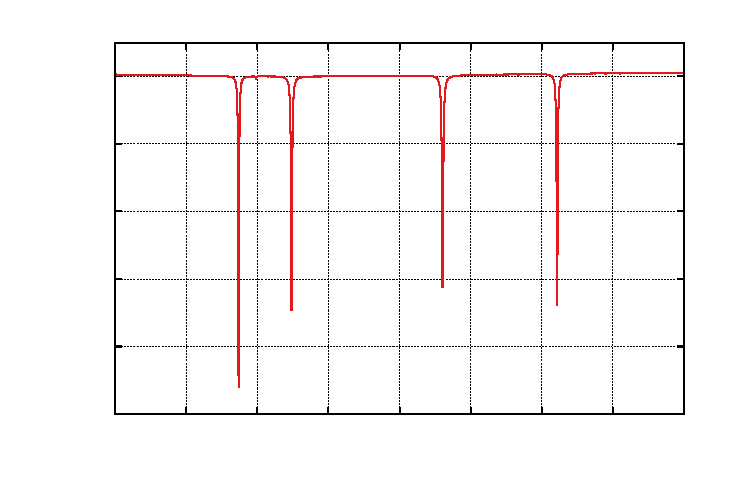
\includegraphics{./plots/spektrum_tm010}}%
    \gplfronttext
  \end{picture}%
\endgroup

	\caption[Reflexionsspektrum der $\mathrm{TM}_{010}$-Moden von PETRA-III]{Reflexionsspektrum der $\mathrm{TM}_{010}$-Moden von PETRA-III. V.\ l.\ n.\ r.: $\pi,\, 2/3~\pi, \, 1/3~\pi$ und $0$-Mode. Bei einer Frequenz von ca.\ \SI{500}{MHz} ist ebenfalls die sehr schwach gekoppelte $5/6~\pi$-Mode erkennbar.}
	\label{fig:spektrum_tm010}
\end{figure}

\begin{figure}[p]
	\centering
	\hspace{2cm} %
	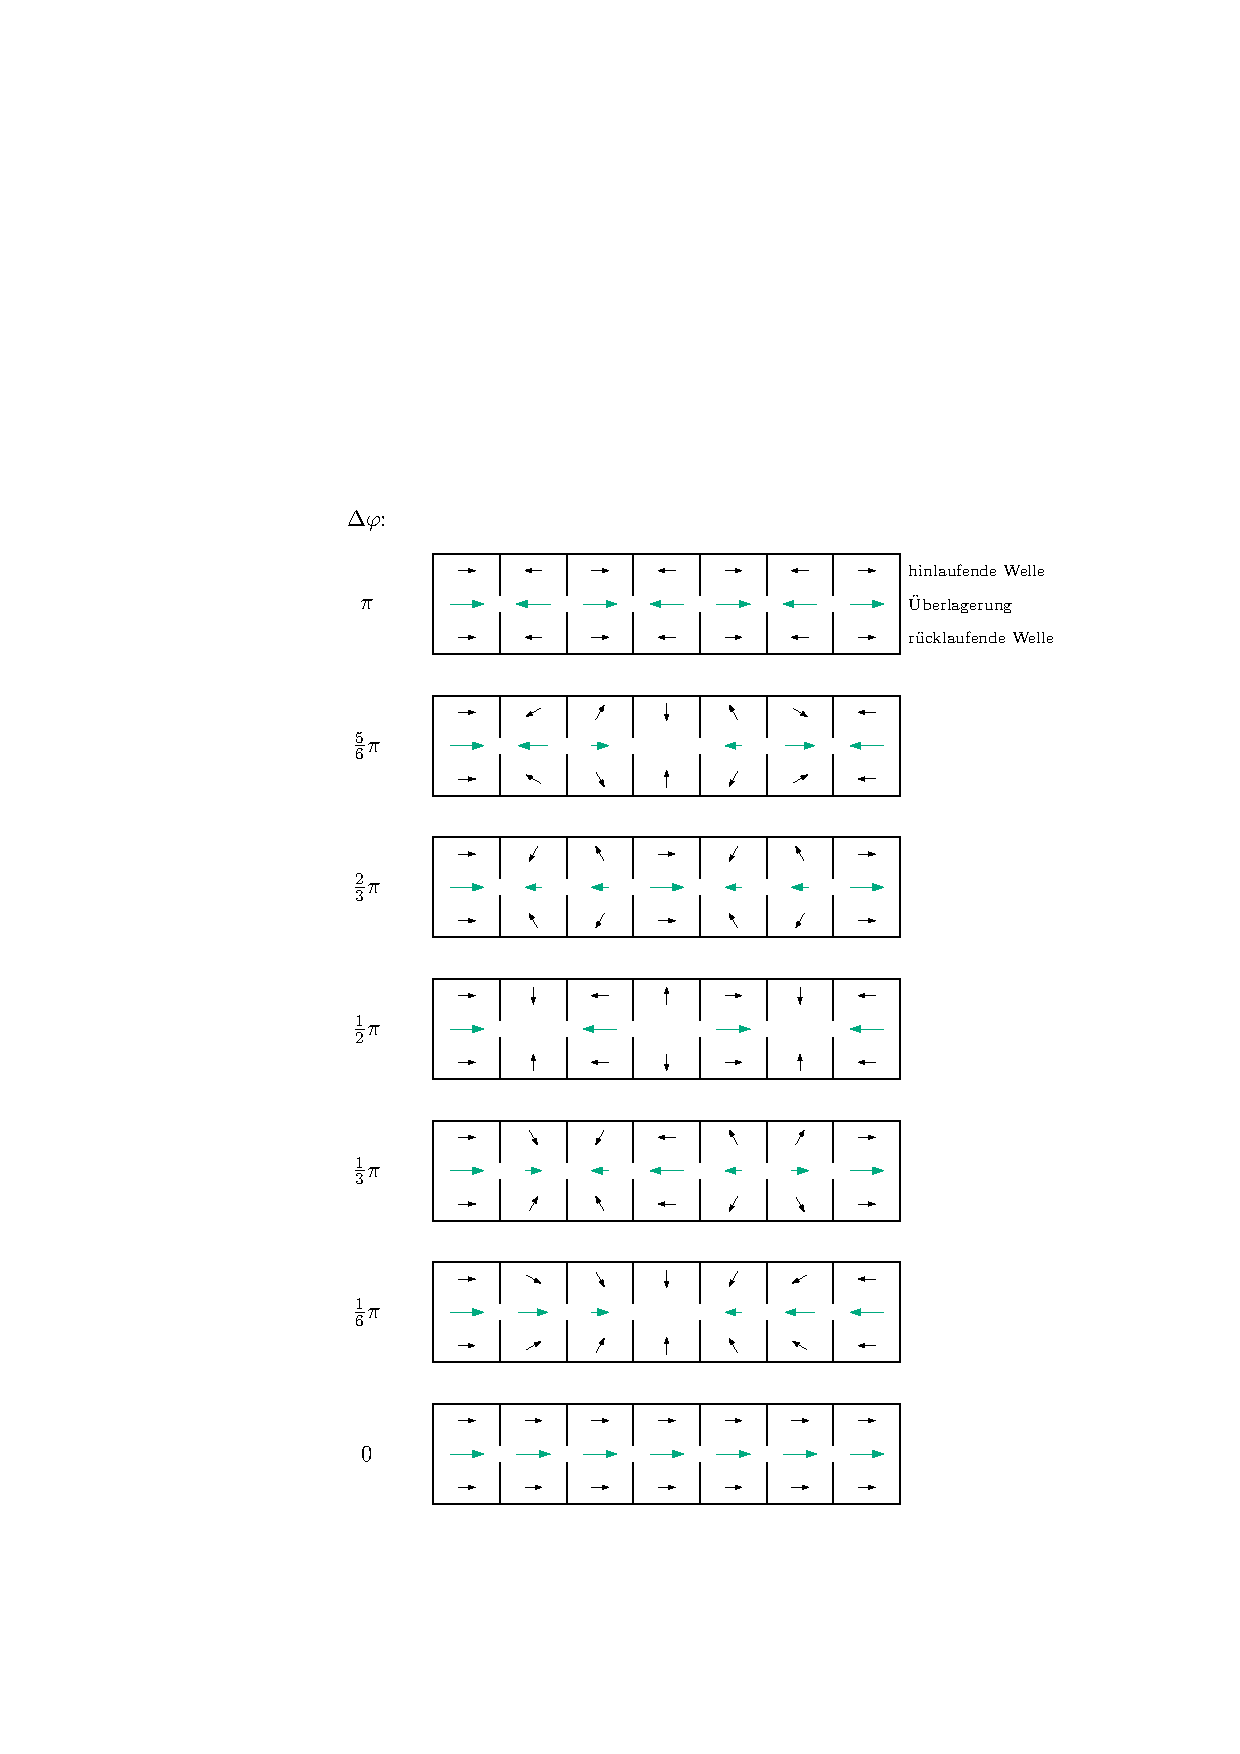
\includegraphics[scale=1.0]{./figs/zellen_phasoren.pdf}
	\caption[Phasenbeziehung in einer siebenzelligen Resonatorkette]{Darstellung der Phasenbeziehung in einer siebenzelligen Resonatorkette durch Überlagerung von hin- und rücklaufender Welle. Amplitude und Phase der einzelnen Komponenten werden als Phasoren dargestellt. Der grüne Phasor kennzeichnet die Überlagerung beider Wellen und zeigt, dass das resultierende Feld nur Phasensprünge von $\pi$ aufweist. Darüber hinaus kommt es in manchen Zellen zur destruktiven Interferenz.}
	\label{fig:phasenbeziehung}
\end{figure}

\begin{figure}[p]
	\centering
	\begin{tabular}{ccc}
		$\Delta \varphi$: &\hspace{1cm}& elektrische Feldverteilung:\\[1.5em]
		$\pi$ &&
		\begin{minipage}{0.7\textwidth}
			\vspace{-1mm}
			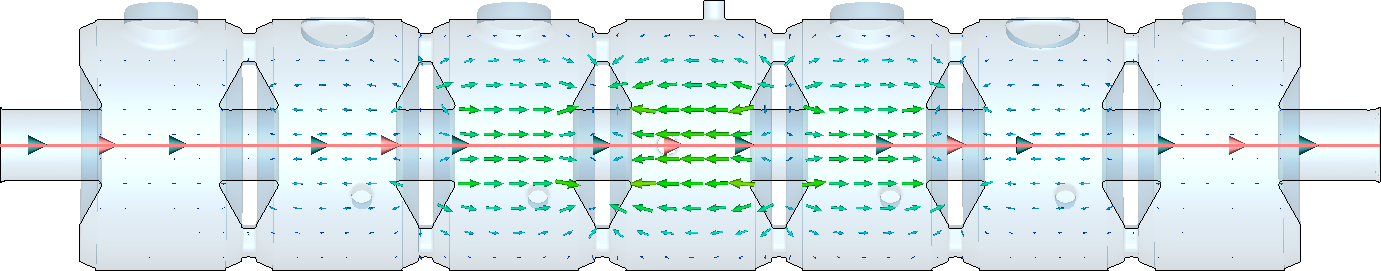
\includegraphics[width=\textwidth]{./figs/TM010-CST/pi_cut.png}
		\end{minipage} \\[3em]
		$\frac{5}{6}\pi$ &&
		\begin{minipage}{0.7\textwidth}
			\vspace{-1mm}
			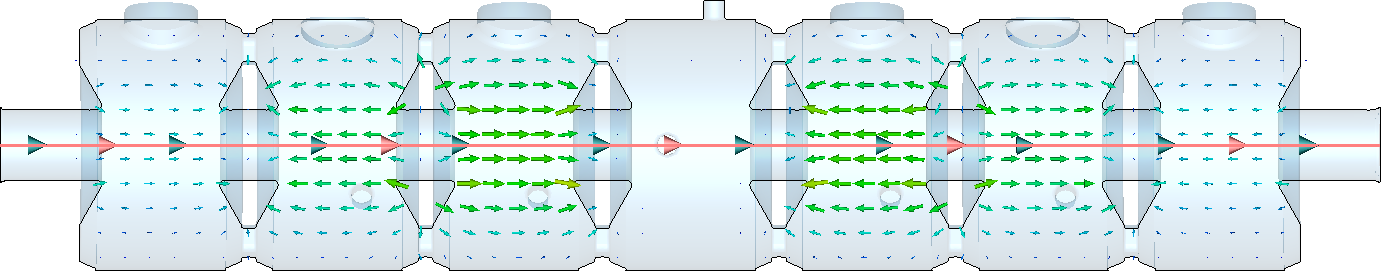
\includegraphics[width=\textwidth]{./figs/TM010-CST/5_6_pi_cut.png}
		\end{minipage} \\[3em]
		$\frac{2}{3}\pi$ &&
		\begin{minipage}{0.7\textwidth}
			\vspace{-1mm}
			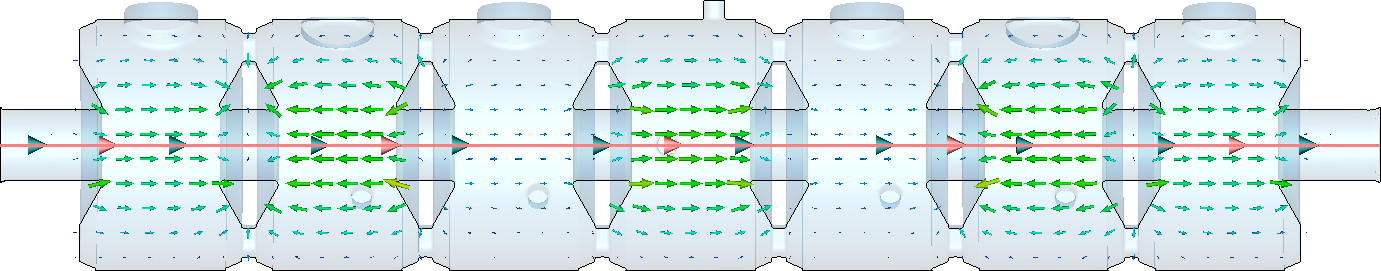
\includegraphics[width=\textwidth]{./figs/TM010-CST/4_6_pi_cut.png}
		\end{minipage} \\[3em]
		$\frac{1}{2}\pi$ &&
		\begin{minipage}{0.7\textwidth}
			\vspace{-1mm}
			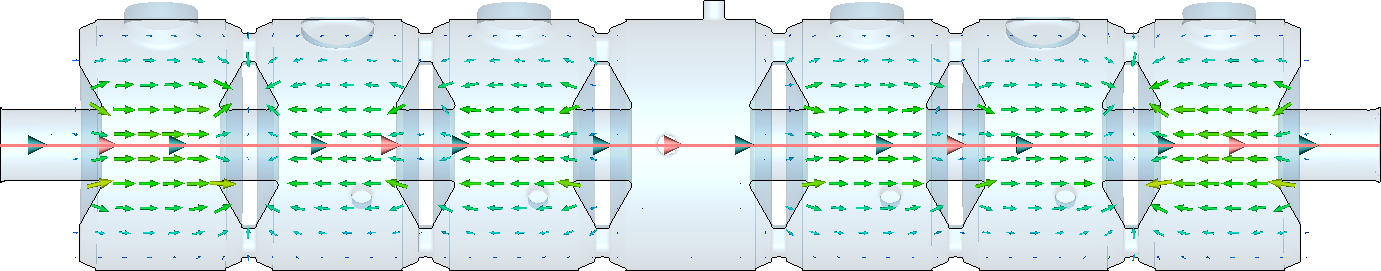
\includegraphics[width=\textwidth]{./figs/TM010-CST/3_6_pi_cut.png}
		\end{minipage} \\[3em]
		$\frac{1}{3}\pi$ &&
		\begin{minipage}{0.7\textwidth}
			\vspace{-1mm}
			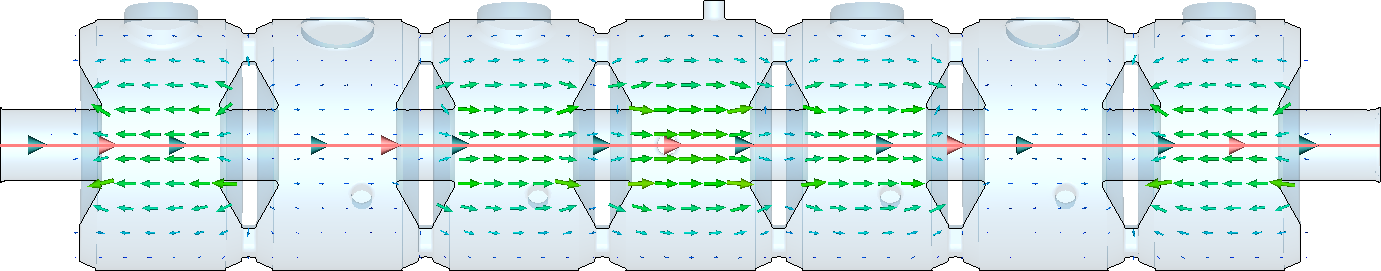
\includegraphics[width=\textwidth]{./figs/TM010-CST/2_6_pi_cut.png}
		\end{minipage} \\[3em]
		$\frac{1}{6}\pi$ &&
		\begin{minipage}{0.7\textwidth}
			\vspace{-1mm}
			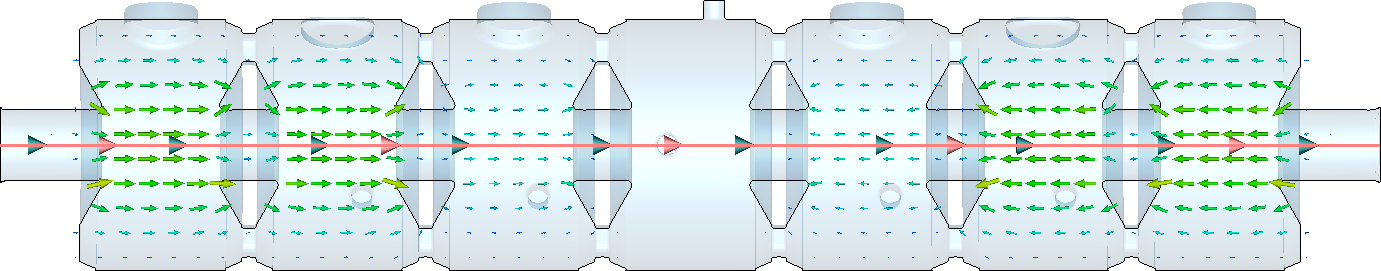
\includegraphics[width=\textwidth]{./figs/TM010-CST/1_6_pi_cut.png}
		\end{minipage} \\[3em]
		$0$ &&
		\begin{minipage}{0.7\textwidth}
			\vspace{-1mm}
			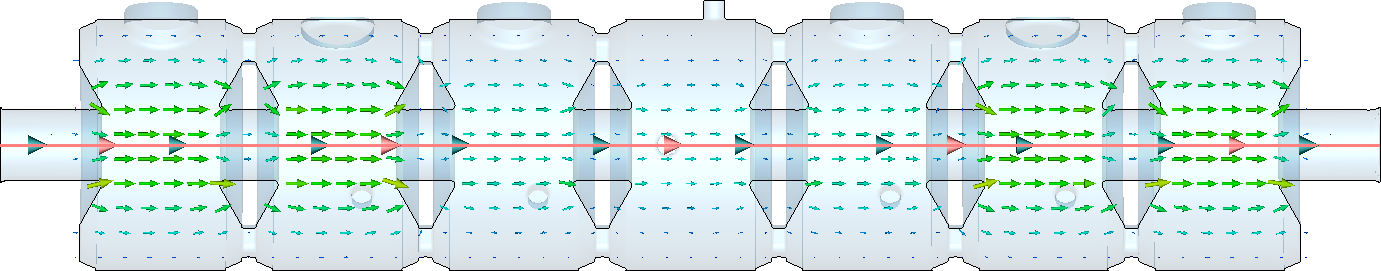
\includegraphics[width=\textwidth]{./figs/TM010-CST/0_cut.png}
		\end{minipage} \\[3em]

	\end{tabular}
	\caption{Simulation der verschiedenen $\mathrm{TM}_{010}$-Eigenmoden eines PETRA-Resonators (die Nose Cones sind nicht vollständig modelliert) mit CST-MWS. Die Pfeile zeigen Richtung, Orientierung und Amplitude des elektrischen Feldes im Resonator zu einem festen Zeitpunkt an.}
	\label{fig:feldverteilung_tm010}
\end{figure}